\chapter{Advanced aircraft CAD modeling}
\label{chapApp1}

In Chapter \ref{chap3} the methodologies and the functions used by \gls{JPAD} to model the aircraft main components have been introduced. Altough these methods help to provide a quite satisfactory representation of the aircraft, it is not enough. More effort can be put in trying to produce functions capable to model additional aircraft parts, such as engines, control surfaces and fairings. This appendix just gives an overview of the tests made in this regard, by providing a description of the adopted methodologies and images of the results. It has to be noted that the functions described in the following are still incomplete and require some work before being actually added to the \gls{JPAD} library.

\section{Wing-Fuselage fairing modeling}
\label{secApp1A1}

Several tests have been performed in order to produce a method providing a satisfactory modeling of the wing to fuselage fairing, whatever the position of one relative to the other. Currently, the method allows to generate ventral fairings (located on the underside of the fuselage, between the main wings) and wing to fuselage fairings in case of high wing, even though still more effort needs to be put on this side in order to obtain decent results. For this reason, the following descriptions and figures refer mostly to the first typology. 

\bigskip
\noindent
Since the \gls{JPAD} aircraft classes do not provide a description for the fairings, all the supporting curves have been designed from scratch, generating the points the curves have to pass through (figures \ref{fig:fairing_01} and \ref{fig:fairing_02}) by means of a set of ad hoc parameters. The fairing generator algorithm currently makes use of the following arguments:
%
\begin{itemize}
\renewcommand\labelitemi{\tiny$\blacksquare$}
\renewcommand\labelitemii{\tiny$\bullet$}
\item \textbf{\lstinline[language=Java]!fuselage!} - An instance of the \gls{JPAD} \lstinline[language=Java]!Fuselage! class, providing all the necessary geometric data regarding the fuselage. 
\item \textbf{\lstinline[language=Java]!wing!} - An instance of the \gls{JPAD} \lstinline[language=Java]!LiftingSurface! class, providing all the necessary geometric data regarding the wing, like its position with respect to the fuselage.
\item \textbf{\lstinline[language=Java]!frontLengthFactor!} - A \lstinline[language=Java]!double! quantity fixing how much the fairing extends forward (in the negative $x$ direction) in terms of lifting surface root chord.
\item \textbf{\lstinline[language=Java]!backLengthFactor!} - A \lstinline[language=Java]!double! quantity fixing how much the fairing extends backward (in the positive $x$ direction) in terms of lifting surface root chord.
\item \textbf{\lstinline[language=Java]!sideSizeFactor!} - A \lstinline[language=Java]!double! quantity standing for how large the fairing should be compared to the fuselage diameter, and currently the code does not allow to make the fairing larger than the fuselage. Besides, in case the lifting surface is not detached from the fuselage, there is a minimum side size that the fairing must respect, in order to be sure it \emph{wraps} the lifting surface, which is the fairing main purpose; this limit is automatically imposed by the code.
\item \textbf{\lstinline[language=Java]!fairingHeightFactor!} - A \lstinline[language=Java]!double! quantity that fixes how much the fairing extends above or below: 
%
\begin{itemize}
\item the fuselage, in case the lifting surface is completely contained in it, 
\item the wing, in case the lifting surface upper/lower surface exceeds the limits imposed by the fuselage. 
\end{itemize}
%
The actual height is then calculated in terms of root chord thickness.
\item \textbf{\lstinline[language=Java]!filletRadiusFactor!} - A \lstinline[language=Java]!double! quantity that fixes the radius of the fillet to be applied to the fairing shapes. The actual radius is obtained by multiplying this factor by the distance between the points A and G shown in figure \ref{fig:fairing_01}, in order to make sure the fillet operation can be actually performed, otherwise the fillet algorithm, provided by the \gls{OCCT} library, would encounter some problematics.
\end{itemize}
%
Other two factors are actually provided to the method but they are not as relevant as the aforementioned ones, or, at least, they could be fixed and excluded from the final fairing function arguments list. These factors are the \textbf{\lstinline[language=Java]!heightBelowContactFactor!} and the \textbf{\lstinline[language=Java]!heightAboveContactFactor!}. The contact to which they make reference is the point in which the fairing, with its side size, actually \emph{touches} the fuselage and crosses its surface. Being the fuselage comparable to some sort of cylinder, two contacts point can be actually distinguished. In order to make sure the fairing is correctly shaped, it is necessary it doesn't exceeds some limits fixed by these contact points. Points A and G in figure \ref{fig:fairing_01} are obtained by the use of these factors. In case of ventral fairing, point G $z$ coordinate value is automatically set greater than the one of the lower contact line (how much greater depends on the value of the \lstinline[language=Java]!heightAboveContactFactor!), but less than the one of the upper contact line, in order for the fairing to not exceeds fuselage limits. Point A $z$ coordinate value, instead, is automatically set less than the one of the lower contact line, but greater than the fuselage lower outline one. The values of these factors are just relevant for the fillet actual radius, since the distance between the points A and G is used as a reference lenght for it.
%
\bigskip
\begin{lstlisting}[caption={Fairing CAD method}, captionpos=b, tabsize=2, label={lst:FairingCADMethod}]
public static List<OCCShape> getFairingShapes(
			Fuselage fuselage, 
			LiftingSurface wing,
			double frontLengthFactor,
			double backLengthFactor,
			double sideSizeFactor,
			double fairingHeightFactor,
			double heightBelowContactFactor,
			double heightAboveContactFactor,
			double filletRadiusFactor
			) {
			...
}
\end{lstlisting}
%
\begin{figure}[H]
\centering
\includegraphics[scale=0.50]{Immagini/Appendice/Fairing/fairing_01}
\caption{Ventral fairing root profile curves}
\label{fig:fairing_01}
\end{figure}
%
\begin{figure}[H]
\centering
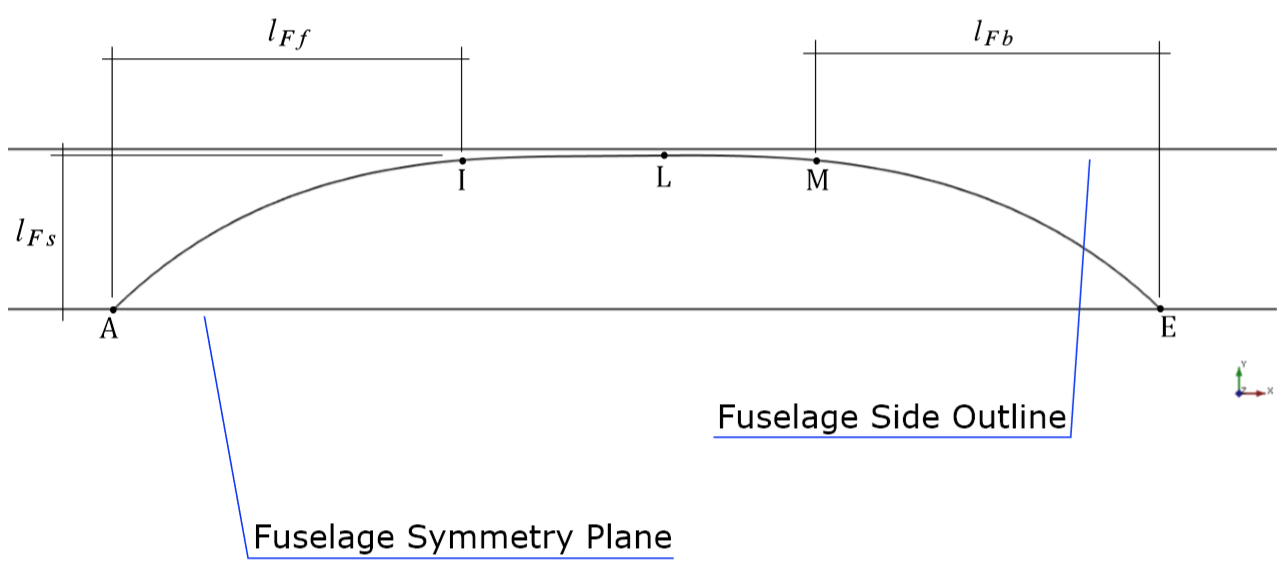
\includegraphics[scale=0.50]{Immagini/Appendice/Fairing/fairing_03}
\caption{Ventral fairing side curve}
\label{fig:fairing_02}
\end{figure}
%  
\bigskip
\begin{table}[H]
\centering
\begin{tabular}{p{1.5cm}p{9.0cm}}
\toprule
\textbf{Length} & \textbf{Description} \\
\midrule
$l_{Ff}$ & The fairing front length, obtained by multiplying the wing root chord by the \lstinline[language=Java]!frontLengthFactor! \\[0.2cm]
$l_{Fb}$ & The fairing back length, obtained by multiplying the wing root chord by the \lstinline[language=Java]!backLengthFactor! \\[0.2cm]
$l_{Fs}$ & The fairing side length, obtained by multiplying half the fuselage width at the wing apex $x$ coordinate by the \lstinline[language=Java]!sideSizeFactor! \\[0.2cm]
$l_{Fh}$ & The fairing height, obtained by multiplying the wing root airfoil thickness by the \lstinline[language=Java]!fairingHeightFactor! \\
\bottomrule
\end{tabular}
\caption{JPAD fairing characteristic lengths}
\label{tab:FairingCharacteristicLengths}
\end{table}
% 

\noindent
By means of the factors listed above, and using the coordinates of the points belonging to the wing root airfoil and the fuselage outlines, the points shown in the previous figures are determined and used in order to generate the wireframe of the fairing. In particular, the side supporting curve depicted in figure \ref{fig:fairing_02} serves as a reference, and is used to build C-shaped elements supporting the following construction of the surfaces belonging to the fairing. In fact, these C-shaped wires, shown in figure \ref{fig:FairingWireframeSupCurves}, extend in the $y$ direction by a quantity provided by the side curve. The edges that form the depicted wires are then used to generate the surfaces of the fairing, by means of the \lstinline[language=Java]!OCCUtils.makePatchThruSections! method (figure \ref{fig:FairingWireframeSupCurves}). It has to be noted that, at this stage, only the right shapes of the fairing are being produced, since the \gls{OCCT} library provides the methods to perform the necessary transformations, as seen in Chapter \ref{chap3}.    
%
\begin{figure}[H]
\centering
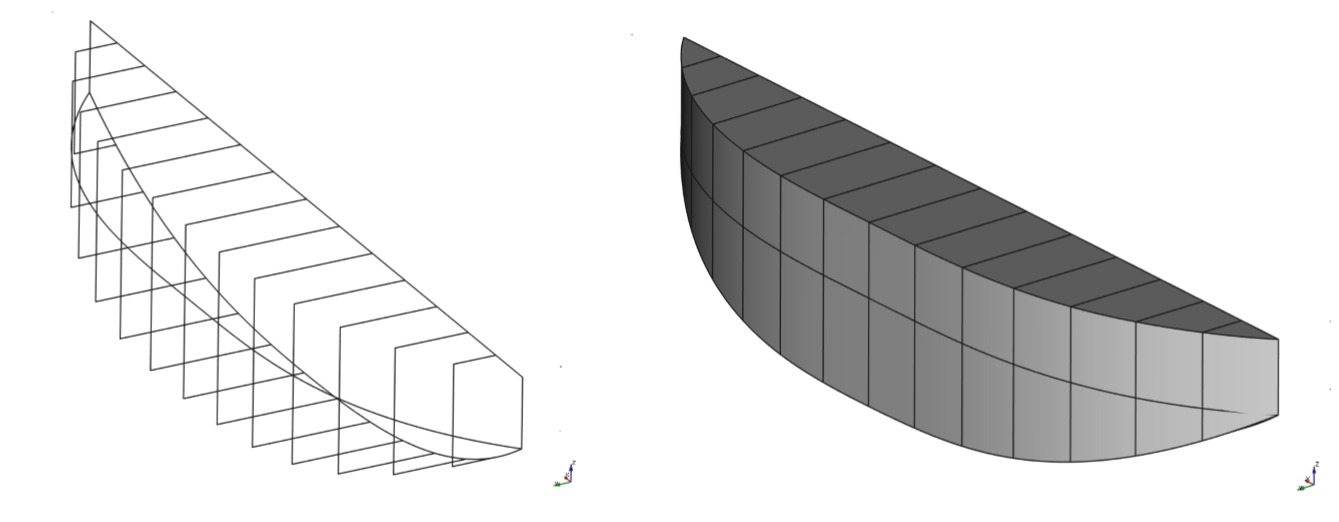
\includegraphics[scale=0.45]{Immagini/Appendice/Fairing/fairing_04}
\caption{Fairing complete wireframe (left) and fairing surfaces (right)}
\label{fig:FairingWireframeSupCurves}
\end{figure}
%  

\bigskip
\noindent
Once the patches on the right side of the fairing have been obtained, they are sewed together by means of the same \gls{OCCT} class used in Chapter \ref{chap3} for the same purpose. The final result is a single shell, onto which a fillet can be applied in order to smooth the edges of the fairing that actually emerge from the fuselage solid. The \gls{OCCT} library provides a class for this operation, called \lstinline[language=Java]!BRepFilletAPI_MakeFillet!, which simply requires the shape on which the operation should be performed, the edge to be smoothed out, and the radius of the fillet. Figure \ref{fig:FairingSolidPlusFillet} shows the final result, once the filleted half fairing shell has been mirrored and the solid has been produced.
%
\begin{figure}[H]
\centering
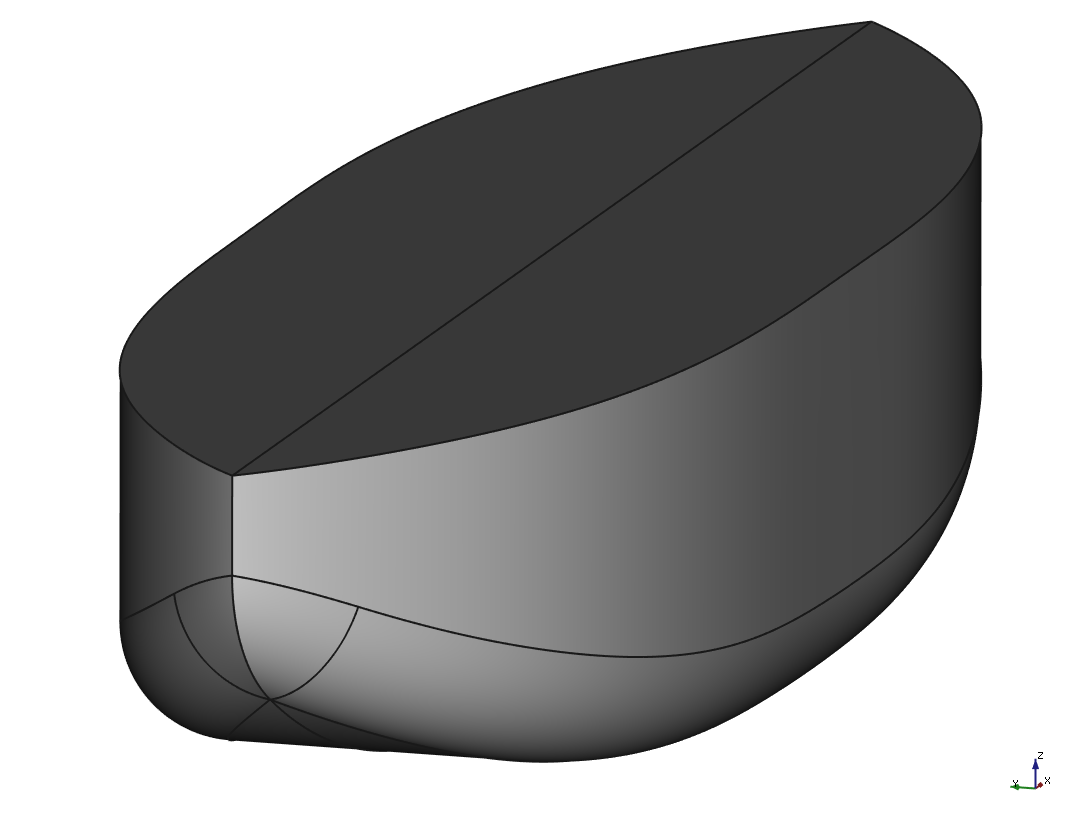
\includegraphics[scale=0.45]{Immagini/Appendice/Fairing/FairingSolidPlusFillet}
\caption{Fairing solid}
\label{fig:FairingSolidPlusFillet}
\end{figure}
%  

\bigskip
\noindent
As mentioned before, the same algorithm can be used to generate different types of fairing. The following pictures show a business aircraft concept equipped with a canard. The function used to generate both the fairings (the one between the canard and the fuselage and the one for the main wing and the fuselage) is exactly the same, with just the values provided to the arguments of the \lstinline[language=Java]!getFairingShapes! function being different (listing \ref{lst:FairingShapes}).
%
\bigskip
\begin{lstlisting}[caption={Fairing CAD method application}, captionpos=b, tabsize=2, label={lst:FairingShapes}]
// Import the aircraft from the XML data file and populate
// JPAD aircraft dedicated classes instances
Aircraft aircraft = AircraftUtils.importAircraft(args);
		
Fuselage fuselage = aircraft.getFuselage();
LiftingSurface wing = aircraft.getWing();
LiftingSurface horTail = aircraft.getHTail();
LiftingSurface verTail = aircraft.getVTail();
LiftingSurface canard = aircraft.getCanard();

// Generate CAD shapes for the aircraft components and the fairings
List<OCCShape> fuselageShapes = getFuselageCAD(
		fuselage, 7, 7, true, true, false);				
List<OCCShape> wingShapes = getLiftingSurfaceCAD(
		wing, ComponentEnum.WING, 1e-3, false, true, false);				
List<OCCShape> wingFairingShapes = getFairingShapes(fuselage, wing,
		1.15, 1.15, 0.50, 0.15, 0.50, 0.50, 0.75);				
List<OCCShape> horTailShapes = getLiftingSurfaceCAD(
		horTail, ComponentEnum.HORIZONTAL_TAIL, 1e-3, false, true, false);				
List<OCCShape> verTailShapes = getLiftingSurfaceCAD(
		verTail, ComponentEnum.VERTICAL_TAIL, 1e-3, false, true, false);				
List<OCCShape> canardShapes = getLiftingSurfaceCAD(
		canard, ComponentEnum.CANARD, 1e-3, false, true, false);				
List<OCCShape> canardFairingShapes = getFairingShapes(fuselage, canard,
		1.50, 0.85, 0.55, 0.20, 0.20, 0.20, 0.75);
\end{lstlisting}
%
\begin{figure}[H]
\centering
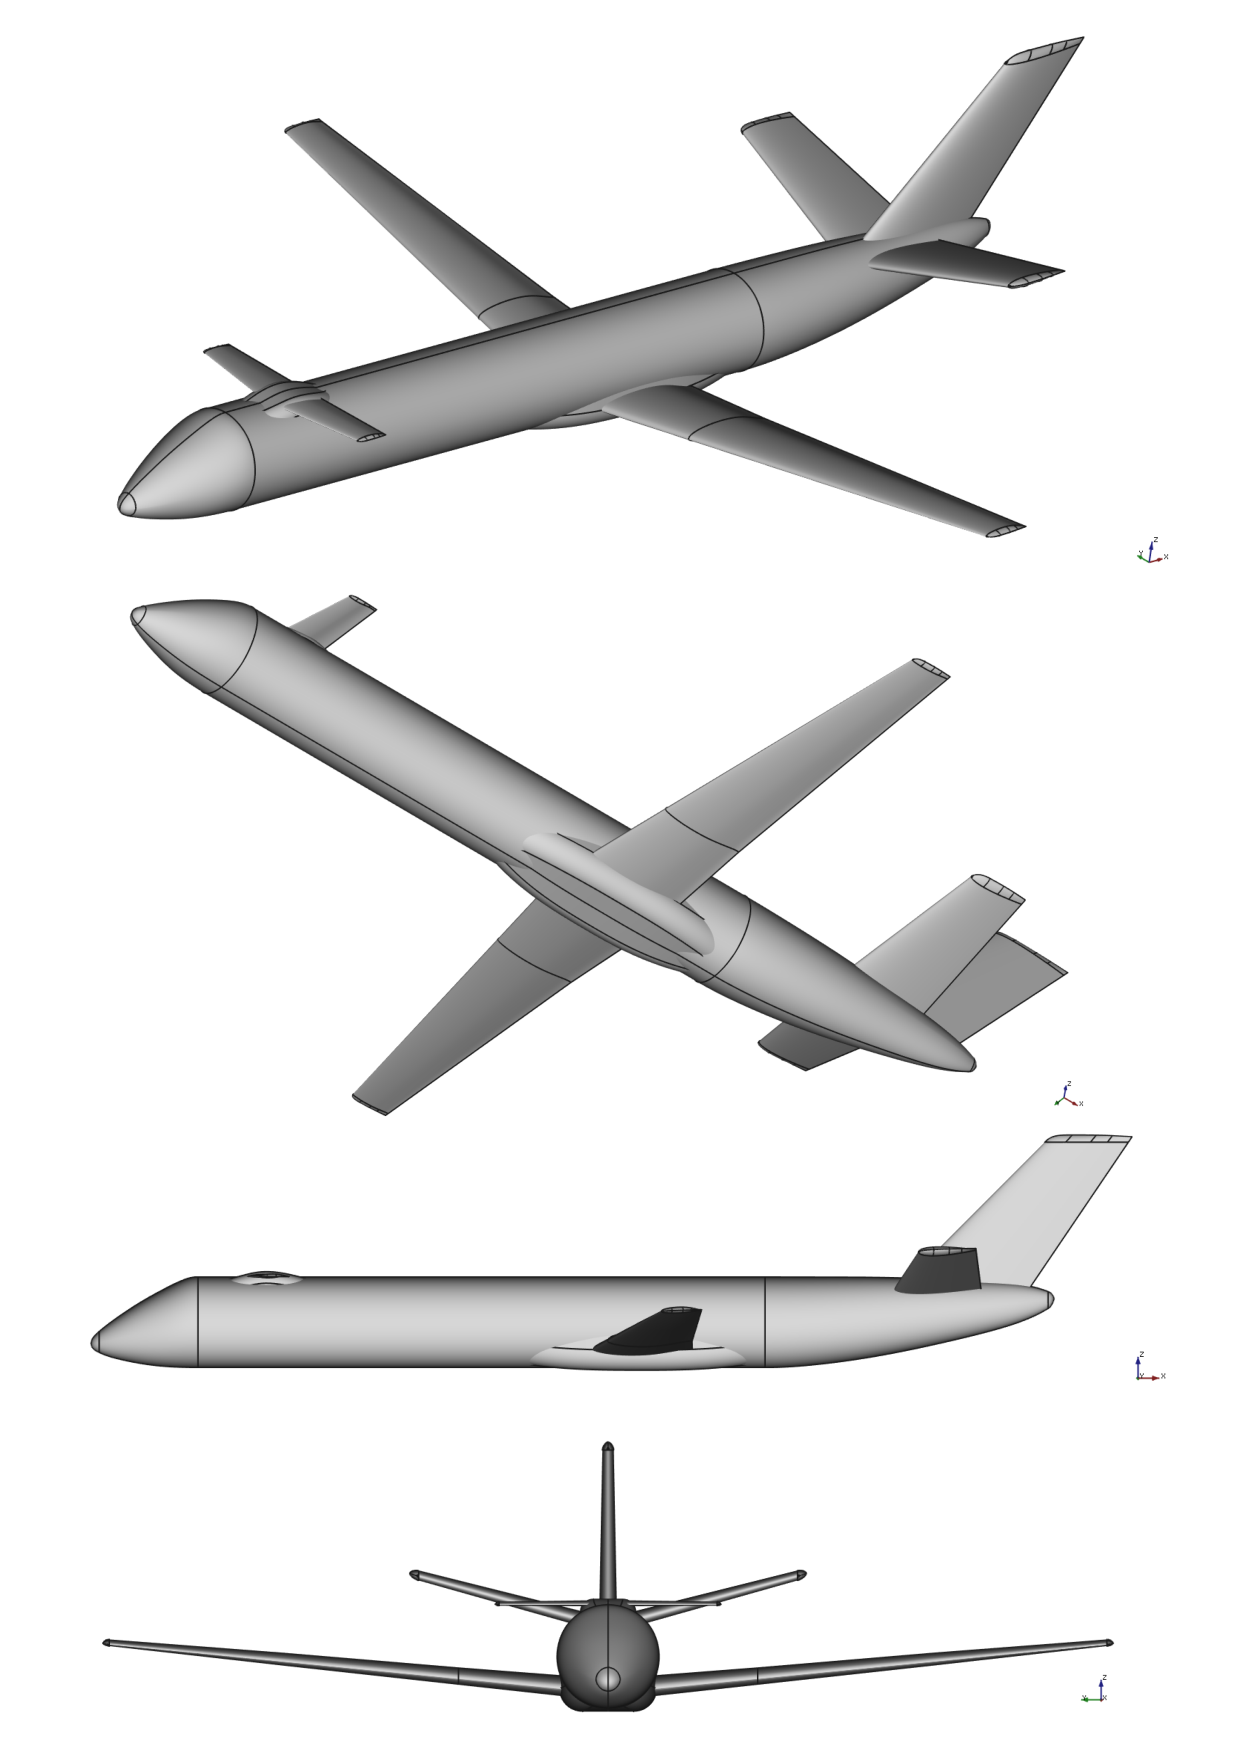
\includegraphics[scale=0.80]{Immagini/Appendice/Fairing/fairing_05}
\caption{Canard and main wing to fuselage fairings}
\label{fig:AircraftFairings}
\end{figure}
%  

\section{Control surfaces modeling}
\label{secApp1A2}

Several tests have been performed in order to evaluate the capabilities of the Boolean operations provided by the \gls{OCCT} library, for the purpose of using the same as the main tool to generate control surfaces. \gls{OCCT}, in fact, comes equipped with a package dedicated to Boolean operations, which is \lstinline[language=Java]!BRepAlgoAPI!, that contains \lstinline[language=Java]!BRepAlgoAPI_Cut!, which is the class providing the methods to perform shell/solid cutting operations. The images and the descriptions below mostly refer to the tests made for Fowler type flaps, altough the same Java code, along with the adopted methodologies, can be easily adapted to generate other typologies of flaps and control surfaces in general.

\bigskip
\noindent
The algorithm implemented in the testing classes first requires a solid shape to begin with, which is generated by the use of the \lstinline[language=Java]!getLiftingSurfaceCAD! methods provided by \lstinline[language=Java]!AircraftUtils!, and the geometric data related to the control surface to be produced, such as the breakpoints and the chords. This data is acquired by the means of the \lstinline[language=Java]!get! methods for symmetric/antysimmetric flaps implemented by  \gls{JPAD} \lstinline[language=Java]!LiftingSurface! class. Then, in order to generate the flapped wing, Boolean operations are needed in order to:
%
\begin{enumerate}
\item generate the cut wing, i.e., the wing once cut but with no flaps;
\item generate the flap itself.
\end{enumerate}
%
These operations require the construction of some dedicated solid entities, which need to be designed from scratch using the data regarding the flaps that has been previously acquired. The first of these \emph{cutting} solids are built by using another \lstinline[language=Java]!BRepAlgoAPI! class, which is \lstinline[language=Java]!BRepAlgoAPI_Section!, that produces a section operation between an argument (the wing solid) and tools (vertical planes lineary distributed along the wing). The result of this operation is a set of airfoils, which can be used in order to produce wires to patch through for the purpose of creating the wing cutting solids (figure \ref{fig:WingCuttingWiresPlusSolid})
%
\begin{figure}[H]
\centering
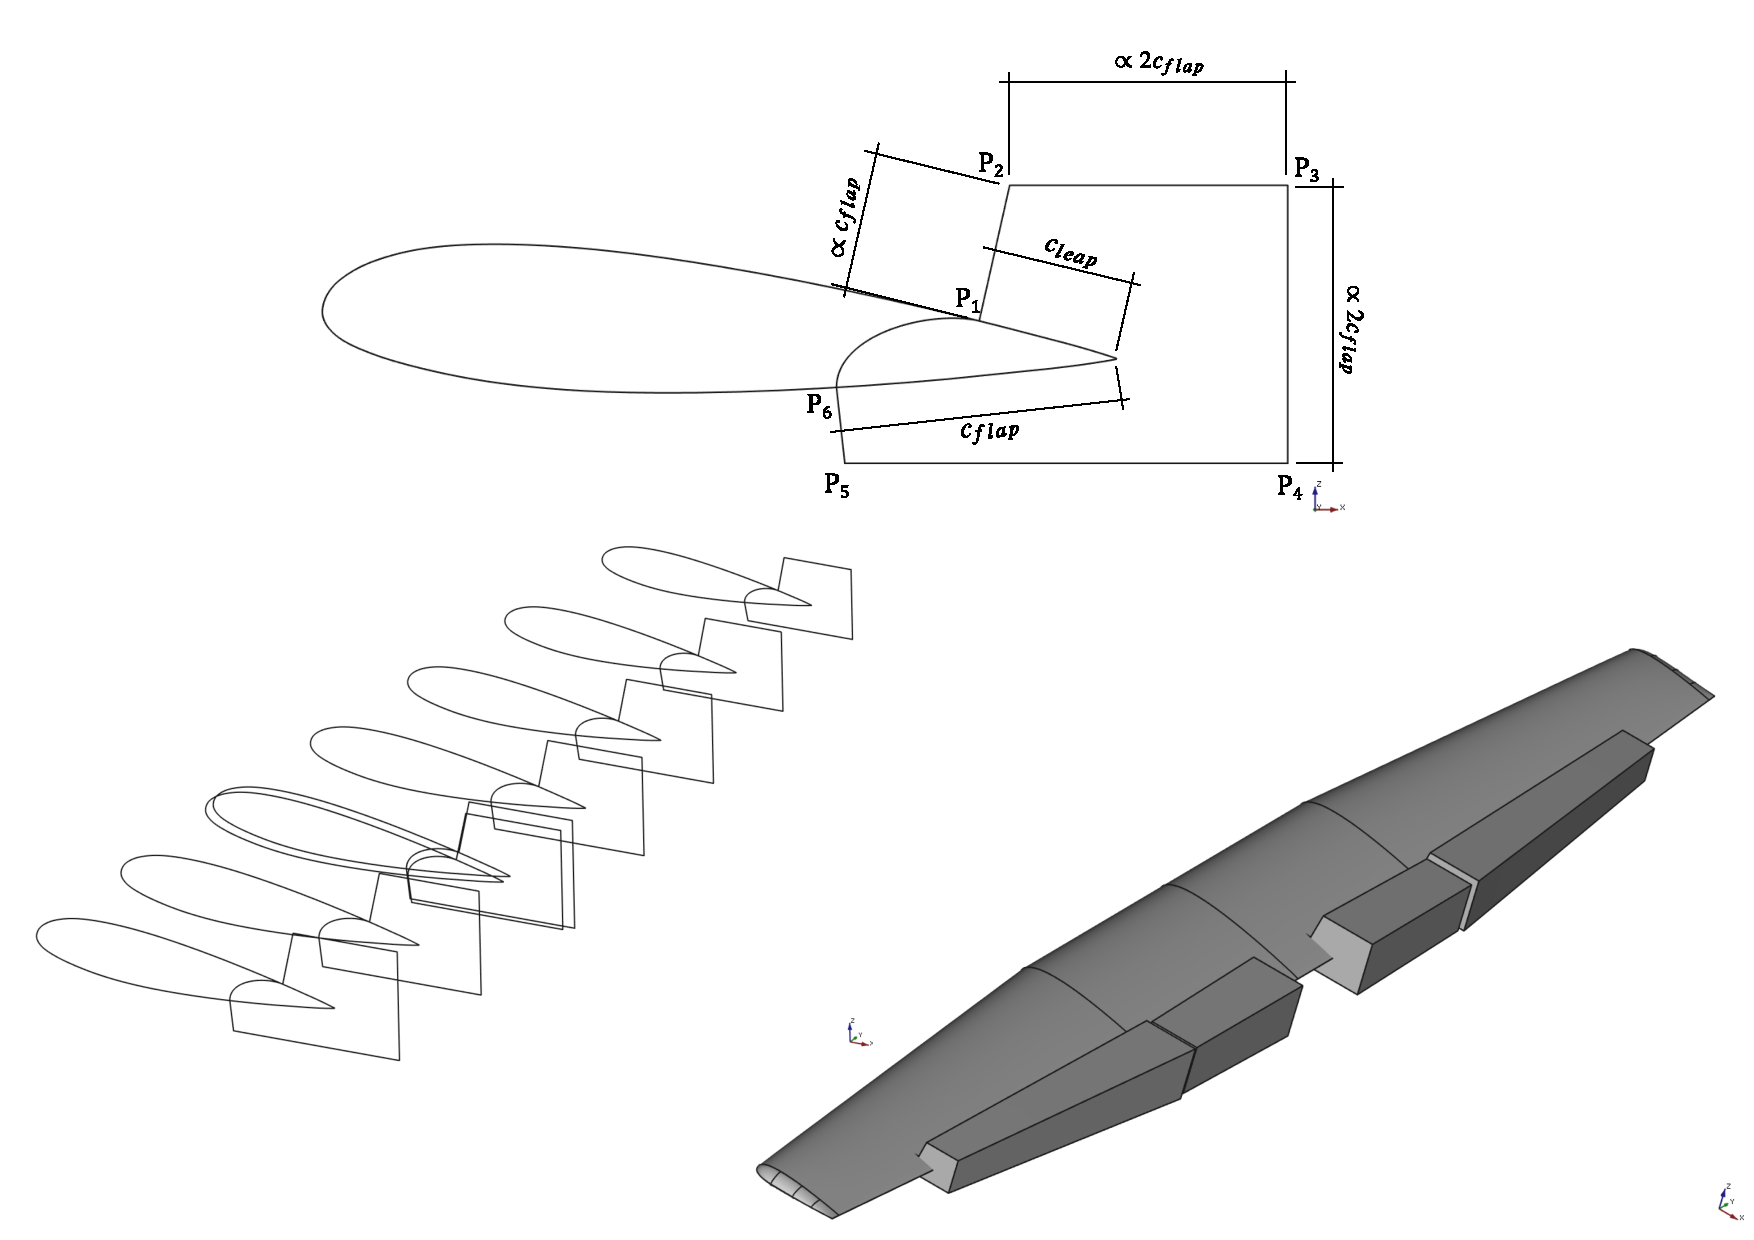
\includegraphics[scale=0.42]{Immagini/Appendice/Flap/flap_05}
\caption{Wing cutting wires (above and left) and wing cutting solids (right) once mirrored}
\label{fig:WingCuttingWiresPlusSolid}
\end{figure}
%  

\bigskip
\noindent
The second set of solids for cutting operations, instead, is produced starting from one of the edges of the wire generated at the previous step, the one that actually intersects the wing shapes. Points are taken on this edge and wires are generated in a similar fashion as the wing cutting ones (figure \ref{fig:FlapCuttingWires}). The solids that result from the patching operation through these wires are used for the flap leading edge adjustment: in fact, the leading edge of the flap must be rounded after the cutting operations for the wing have been performed. This operation could actually be avoided by using the functionalities provided by the \lstinline[language=Java]!BRepFilletAPI_MakeFillet! class instead, as seen for the fairing. But some problems could arise during the filleting operations in case a double edge has been generated at the flap leading edge by the Boolean cut executed on the wing. In order to prevent this possibility, the code performs the rounding of the leading edge of the flap in the aforementioned manner.
%
\begin{figure}[H]
\centering
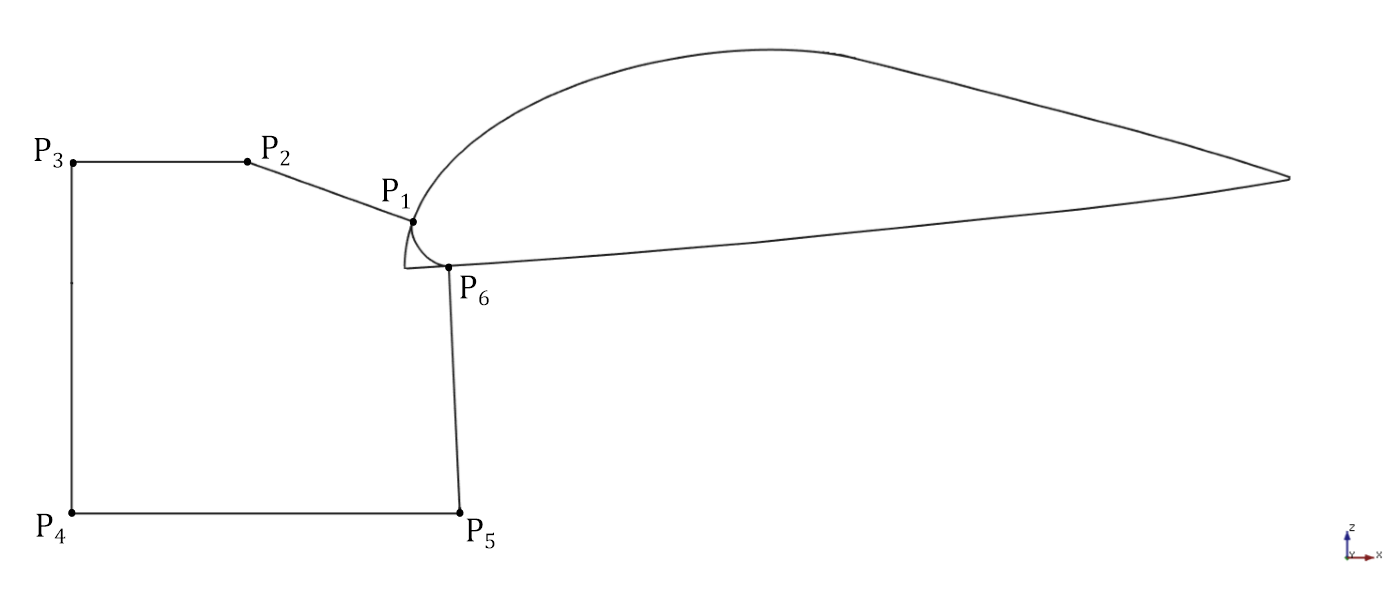
\includegraphics[scale=0.40]{Immagini/Appendice/Flap/flap_08}
\caption{Flap cutting wire}
\label{fig:FlapCuttingWires}
\end{figure}
%  

\bigskip
\noindent
Once the supporting solids have been produced, Boolean cutting operations can be finally executed. First, cuts are performed on the wing by subtracting wing cutting solids from it one by one. At the end of each cut the argument of the Boolean operation is updated, in order to obtain the so-called cut wing (figure \ref{fig:CutWing}). Turning to the flaps, auxiliary cut wings must be created first (at the center in figure \ref{fig:WingAuxCutWingFlap}). These solids are generated at the same way of the previous ones, but without updating the argument of the Boolean operation, so that it stays equal to the original wing. Then the auxiliary cut wings are subtracted one by one from the wing, in order to obtain the flaps, whose leading edge is adjusted by means of the aforementioned flap cutting solids (figure \ref{fig:FlapLEAdjustment}).
%
\begin{figure}[H]
\centering
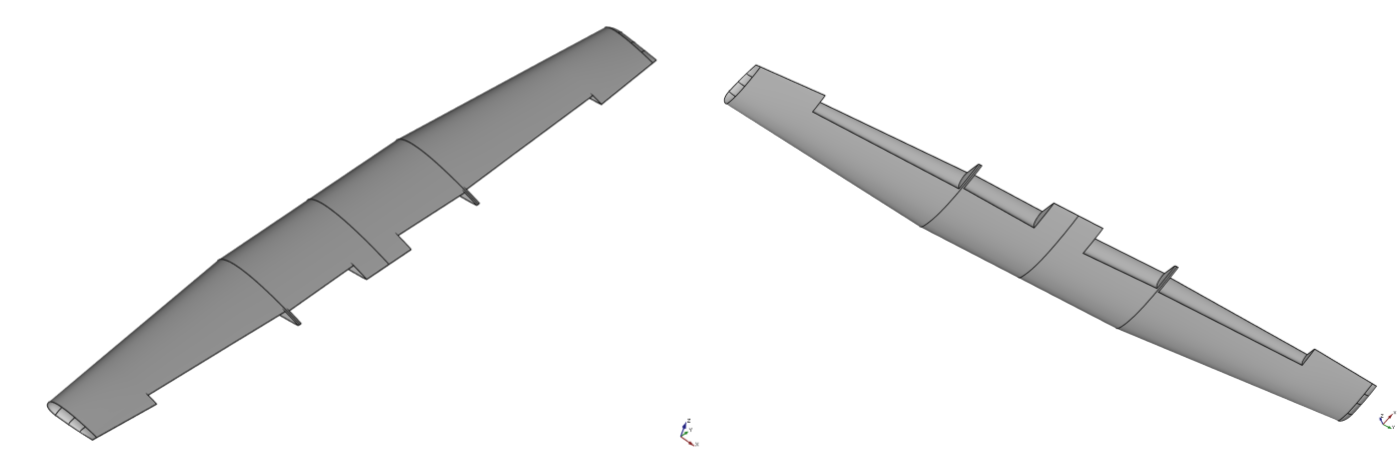
\includegraphics[scale=0.52]{Immagini/Appendice/Flap/WingCutSolid_04}
\caption{Cut wing}
\label{fig:CutWing}
\end{figure}
%
\begin{figure}[H]
\centering
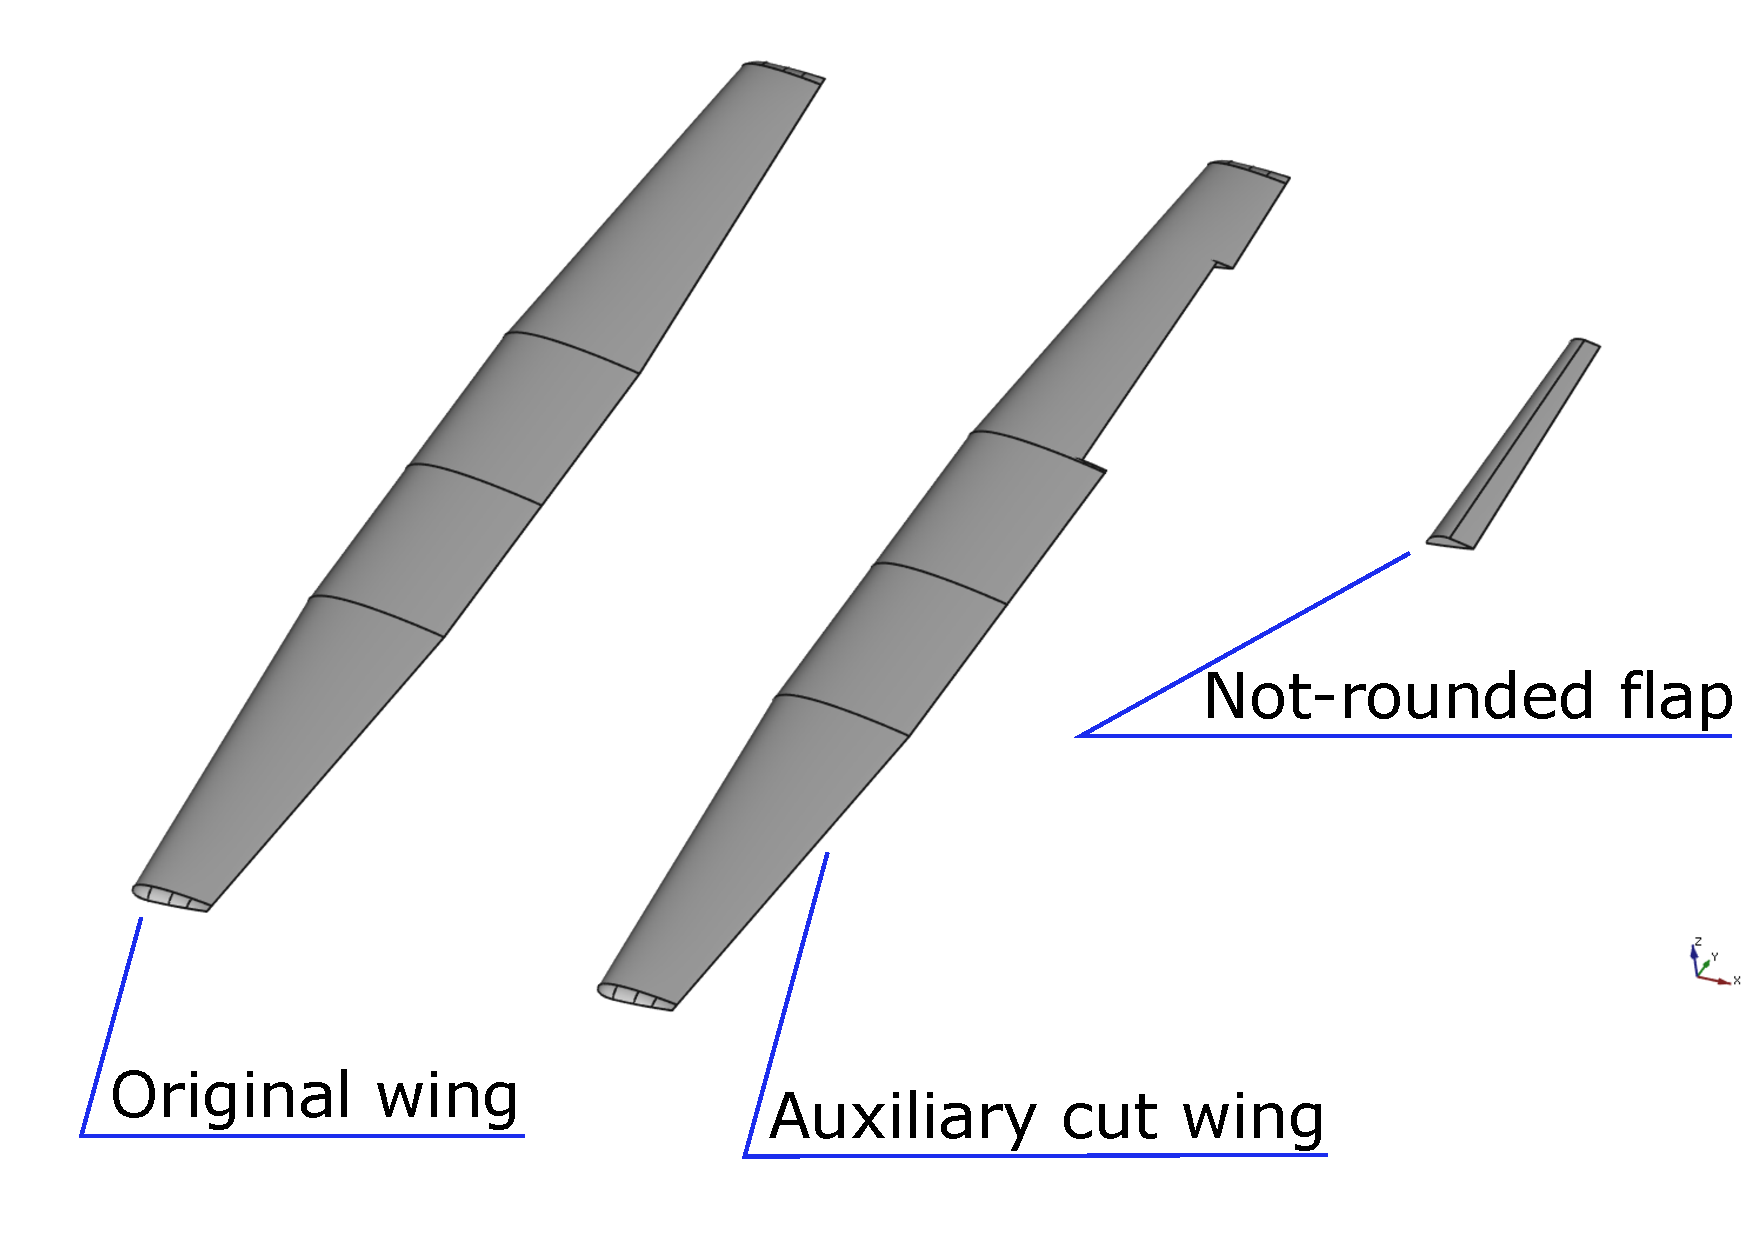
\includegraphics[scale=0.50]{Immagini/Appendice/Flap/flap_07}
\caption{Flap generation steps}
\label{fig:WingAuxCutWingFlap}
\end{figure}  
%
\begin{figure}[H]
\centering
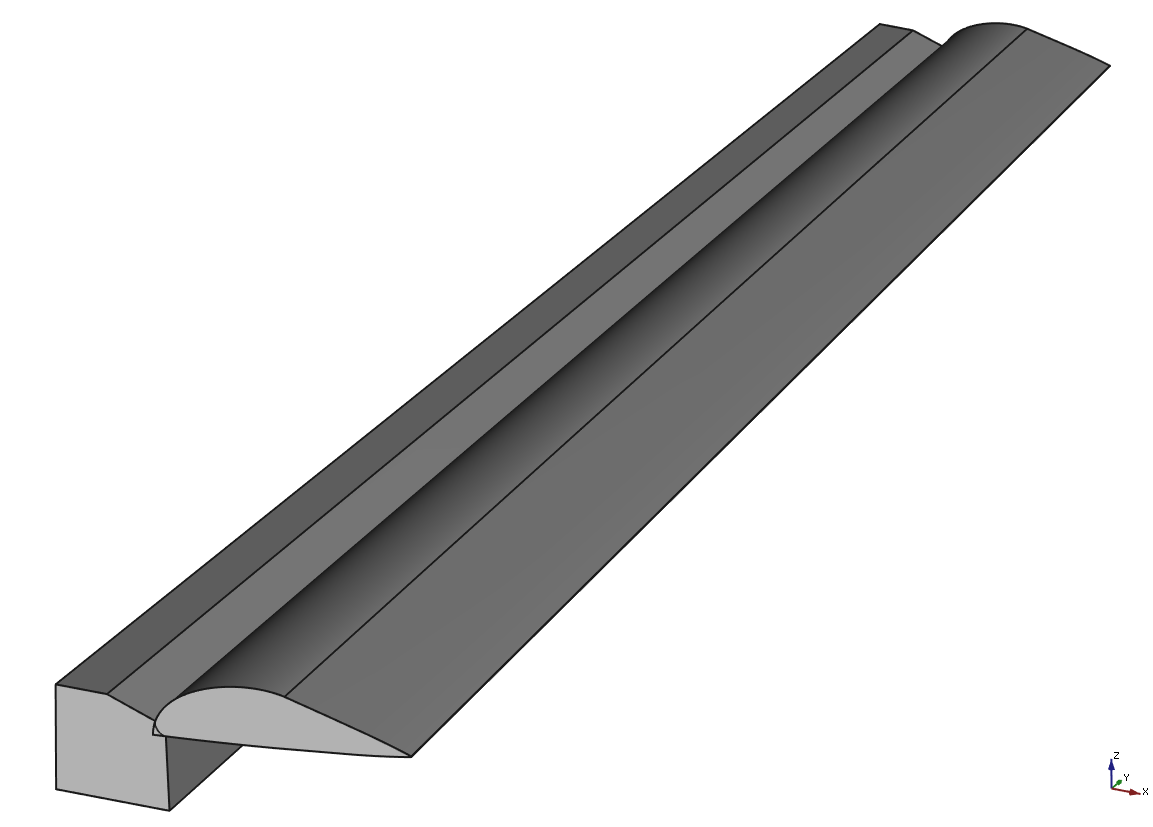
\includegraphics[scale=0.35]{Immagini/Appendice/Flap/FlapPlusFlapCuttingSolid_01}
\caption{Flap leading edge adjustment}
\label{fig:FlapLEAdjustment}
\end{figure}
%  

\bigskip
\noindent
The final step consists in moving the flaps with respect to the cut wing. As mentioned before, the \gls{OCCT} library provides also the classes to perform transformations such as translation and rotation. However, it has to be noted that the current algorithm for control surfaces motion still needs some work and adjustment, especially regarding the Fowler flaps. The following figures show the final result for different wings. In particular, figures \ref{fig:ATR72Fowler} and \ref{fig:CS300Fowler} show the wings of the ATR-72 and CS300 respectively, equipped with inboard and outboard Fowler flaps. Figure \ref{fig:TailControlSurfaces}, instead, shows the horizontal and vertical stabilizers of the ATR-72, equipped with elevator and rudder treated as plain flaps.
%
\begin{figure}[H]
\centering
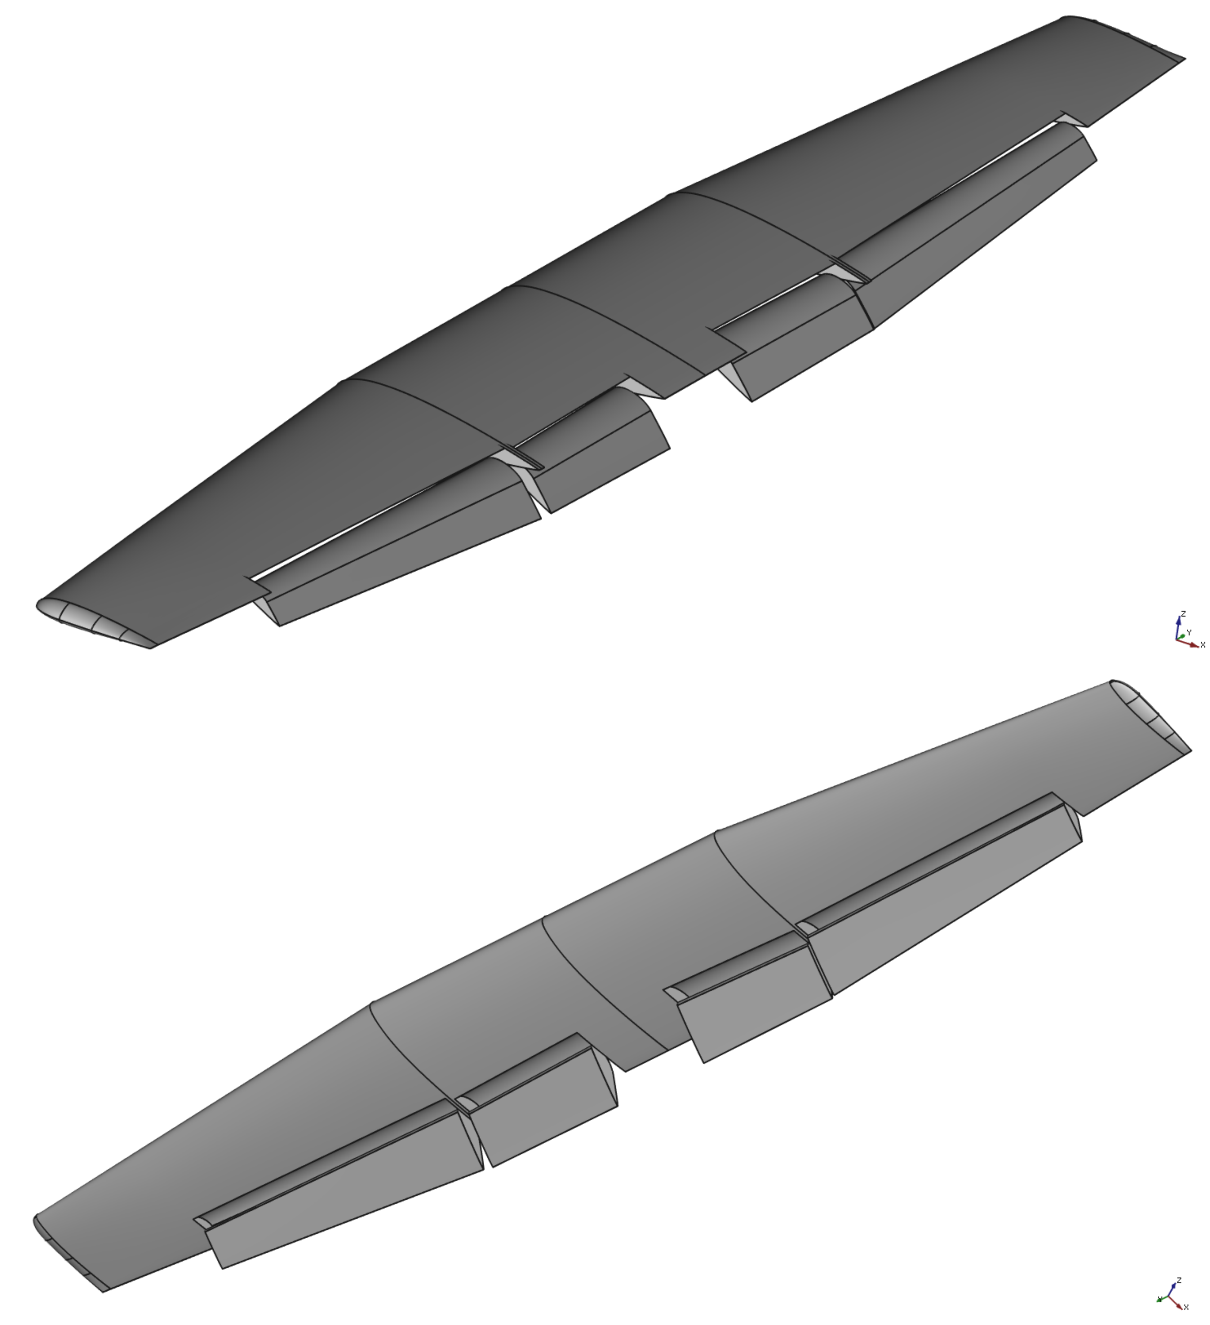
\includegraphics[scale=0.50]{Immagini/Appendice/Flap/flap_09}
\caption{ATR-72 wing, with inboard and outboard Fowler flaps}
\label{fig:ATR72Fowler}
\end{figure}
%
\begin{figure}[H]
\centering
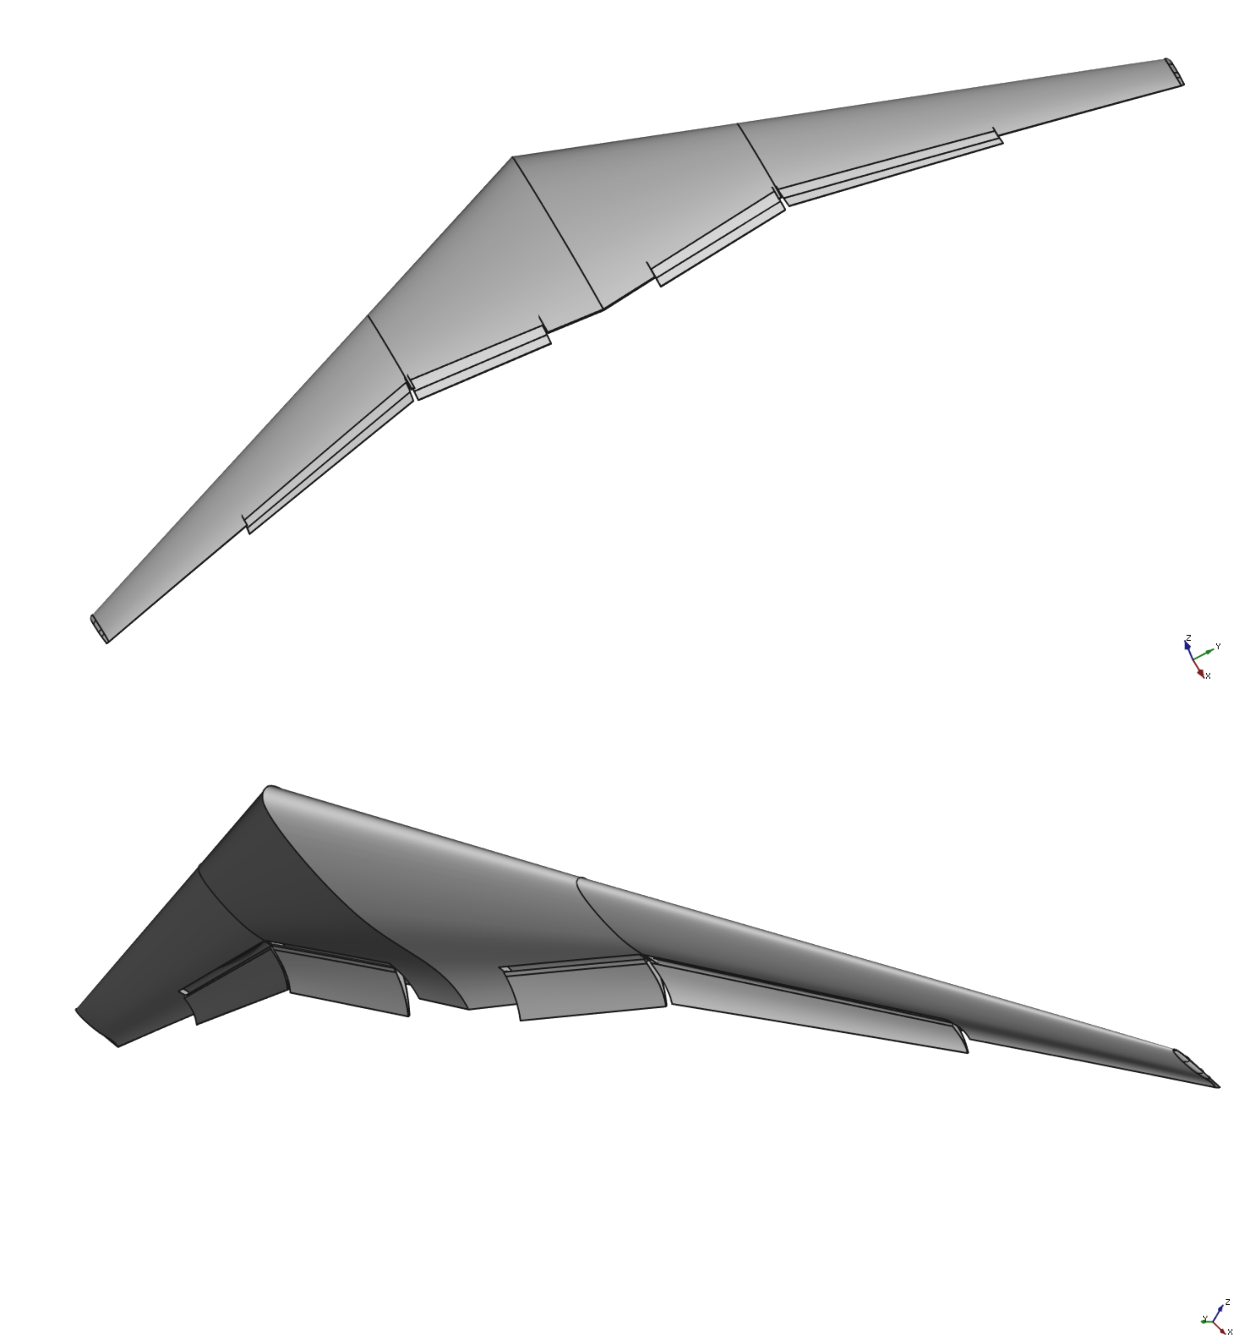
\includegraphics[scale=0.50]{Immagini/Appendice/Flap/flap_10}
\caption{CS300 wing, with inboard and outboard Fowler flaps}
\label{fig:CS300Fowler}
\end{figure}
%
\begin{figure}[H]
\centering
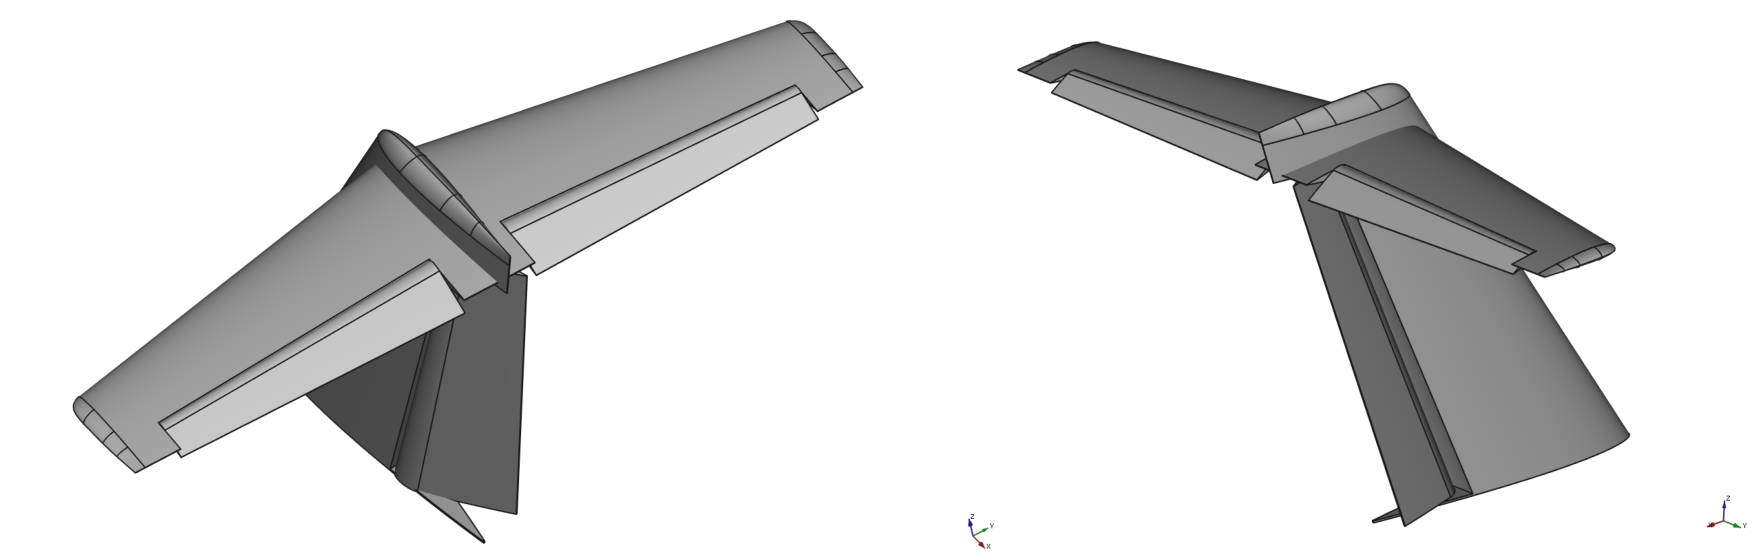
\includegraphics[scale=0.50]{Immagini/Appendice/Flap/flap_11}
\caption{ATR-72 tail, with rotated elevator and rudder}
\label{fig:TailControlSurfaces}
\end{figure}
%